\newsavebox{\PreviewPairedGraphic}
\begingroup
\makeatletter
\let\PreviewEndFloatBox\@endfloatbox
\def\@endfloatbox{\PreviewEndFloatBox
\typeout{FIVE-FLOAT-HEIGHT=\the\ht\@currbox}
\typeout{FIVE-FLOAT-DEPTH=\the\dp\@currbox}}
\makeatother
\begin{figure}[t]
  \centering
  \sbox{\PreviewPairedGraphic}{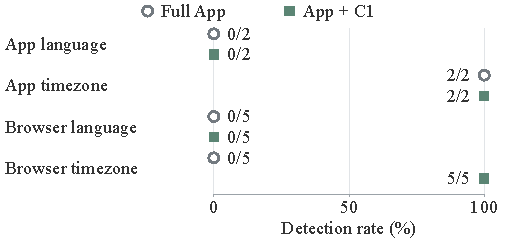
\includegraphics[width=\linewidth]{figures/F05a_main.pdf}}
\typeout{FIVE-TEXTWIDTH=\the\textwidth}
\typeout{FIVE-COLUMNWIDTH=\the\columnwidth}
\typeout{FIVE-TEXTHEIGHT=\the\textheight}
\typeout{FIVE-GRAPHIC-WIDTH=\the\wd\PreviewPairedGraphic}
\typeout{FIVE-GRAPHIC-HEIGHT=\the\ht\PreviewPairedGraphic}
\typeout{FIVE-GRAPHIC-DEPTH=\the\dp\PreviewPairedGraphic}
\usebox{\PreviewPairedGraphic}
  \caption{Full App and App + C1 (accepted cross-endpoint timezone check) on 60 saved development positions: 14 interventions, 46 normal. Points show detection rates with T/N labels. C1 adds Browser timezone detection; language edits remain undetected. Three frozen configurations share counts without pooling denominators. Both methods have 0/46 normal alarms. This is not a new blind test; broader normal costs are reported separately.}
  \Description{Four intervention rows compare Full App, shown as upper hollow gray circles, with App plus the accepted cross-endpoint timezone check C1, shown as lower filled gray-green squares. Exact T/N labels accompany eight points on a zero-to-one-hundred-percent detection axis. Browser timezone changes gain detection from zero of five to five of five. App timezone detection remains two of two, and both language groups remain undetected. Normal alarms are reported separately in the caption.}
  \label{fig:paired-timezone-gain}
\end{figure}
\endgroup
